\documentclass[twoside,12pt]{article}
\usepackage{light, graphicx, subfigure}

%\hidesolutions
\showsolutions

\begin{document}

\problemset{1}{September 9, 2010}{Monday, September 13}
\begin{problem}{15}
Let $G = (V,E)$ be a graph. A {\em matching} in $G$ is a set $M \subset E$ such that no two edges in $M$ are incident on a common vertex.

Let $M_1$, $M_2$ be two matchings of $G$. Consider the new graph $G' = (V, M_1 \cup M_2)$ (i.e. on the same vertex set, whose edges consist of all the edges that appear in either $M_1$ or $M_2$). Show that $G'$ is bipartite.

We will need this result in one of the coming lectures.

\solution{
% Jay Writes:
%The solution to 1 needs to be revised to better handle 2-cycles.  For example
%(e_1, e_2) is a 2-cycle if e_1 = e_2.  In this case both e_1 and e_2 would be
%in M_1.

We will show that $G'$ has no odd cycle. By the theorem proved in recitation (that a graph is bipartite iff it has no odd cycles) we will be done.

First, consider any vertices connected by an edge that is in both $M_1$ and $M_2$.  Since these are matchings, there is no other edges connected to these vertices in either $M_1$ or $M_2$ and thus $G'$. These vertices form connected components of size two which have no odd length cycles.  For the rest of the proof, we can assume that every edge in $G'$ came from exactly one of $M_1$ or $M_2$.

Take a sequence of edges $(e_1, e_2, \ldots, e_k)$ in $G'$ that form a cycle. Let us show that $k$ must be even. We know that $e_1 \in M_1 \cup M_2$. Assume $e_1 \in M_1$ (otherwise $e_1 \in M_2$ and the argument is identical replacing $M_1$ with $M_2$). Now since $e_1$ and $e_2$ are incident on a common vertex, and $M_1$ is a matching, $e_2$ cannot be in $M_1$. So $e_2\in M_2$. Similarly $e_3 \in M_1$, $e_4 \in M_2$ etc. By induction we can prove that for all $i \leq k$, $e_i \in M_1$ iff $i$ is odd.

Now if $k$ had been odd, we would have $e_k \in M_1$. But $e_k$ and $e_1$ are adjacent edges in the cycle, and hence incident on a common vertex, we have a contradiction. Thus $k$ must be even.
}
\end{problem}
\begin{problem}
Let $G = (V,E)$ be a graph. Recall that the {\em degree} of a vertex $v \in V$, denoted $d_v$, is the number of vertices $w$ such that there is an edge between $v$ and $w$.
\begin{itemize}
\item Prove that $$2|E| = \sum_{v\in V} d_v.$$
\solution{
Let $S = \{(e,v) \in E \times V: e \mbox{ is incident on } v \}$.

Count the elements in $S$ as follows
$$|S| = \sum_{e \in E} |\{v: (e,v) \in S\}| = 2 |E|$$
and also as
$$ |S| = \sum_{v \in V} |\{e: (e,v) \in S\}| = \sum_{v\in V} d_v.$$
The result follows.

Once can also prove it by induction on $|E|$. You should try to.
 }
\item At a 6.042 ice-cream study session (where ice-cream flows by the way, really, you should go ... and yeah, it helps you study too) 111 students showed up. During the session, some students shook hands with each other (everybody being happy and content with the ice-cream and all). Turns out that the University of Chicago did another spectacular study here, and counted that each student shook hands with exactly 17 other students. Can you debunk this too?
\solution{ Assume that the study is accurate. Define a graph $G=(V,E)$ with students as vertices and put an edge between 2 students if they shook hands. By the previous problem, we should have $2|E| = \sum_{v} d_v = 111\cdot 17$. But the LHS is even and the RHS is odd, a contradiction.}
\item And on a more dull note, how many edges does $K_n$, the complete graph on $n$ vertices, have?
\solution{
Apply the first part of the problem. Notice that each vertex is joined to $n-1$ others.
$2|E| = \sum_{v}d_v = n(n-1)$. So $|E| = n(n-1)/2$.}
\end{itemize}


\end{problem}
\begin{problem}{20}
The most famous application of stable matching was in assigning
graduating medical students to hospital residencies.  Each hospital has a
preference ranking of students and each student has a preference order of
hospitals, but unlike the setup in the notes where there are an equal
number of boys and girls and monogamous marriages, hospitals generally have
differing numbers of available residencies, and the total number of
residencies may not equal the number of graduating students.  Modify the
definition of stable matching so it applies in this situation, and explain
how to modify the Mating Ritual so it yields stable assignments of students
to residencies.  No proof is required.

\solution{
The Mating Ritual can be applied to this situation by letting the students
be the boys and each of the \emph{residencies} (not the hospitals) be the
girls.

A matching is an assignment of students to residencies (an injection, $A:
\text{students} \to \text{residencies}$) such that every student has a
residency ($A$ is total), or every residency has an assigned student ($A$
is a surjection).  A stable assignment is one with no \emph{rogue couples},
where a rogue couple is a hospital student pair $(H,S)$ such that $S$ is
not assigned to one of the residencies at $H$, which she prefers over
her current assignment, and
\begin{itemize}
\item $H$ has some students assigned to some of its residencies and
prefers $S$ to at least one of its assigned students, or

\item $H$ has none of its residencies assigned,

\end{itemize}

}

\end{problem}

\begin{problem}{10}
% \iffalse
% Last used S06, ps4;
% used F06: Essentially taken from the Course Notes for the
% University of Waterloo class C&O 230.
% \fi

A property of a graph is said to be \emph{preserved under isomorphism} if
whenever $G$ has that property, every graph isomorphic to $G$ also has
that property.  For example, the property of having five vertices is
preserved under isomorphism: if $G$ has five vertices then every graph
isomorphic to $G$ also has five vertices.

Determine which among the four graphs pictured in the Figures 
%~\ref{fig:isog}
are isomorphic.  If two of these graphs are isomorphic, describe an
isomorphism between them.  If they are not, give a property that is
preserved under isomorphism such that one graph has the property, but the
other does not.  For at least one of the properties you choose,
\emph{prove} that it is indeed preserved under isomorphism (you only need
prove one of them).

\begin{figure}[h] %[htbp]
\begin{center}
\mbox{  \subfigure[$G_1$]{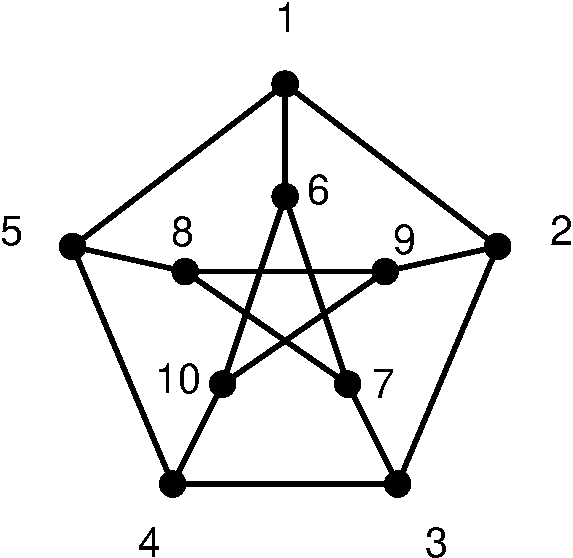
\includegraphics[width=1.5in,clip]{latex-macros/figures/G1}}
        \hspace{17mm}
        \subfigure[$G_2$]{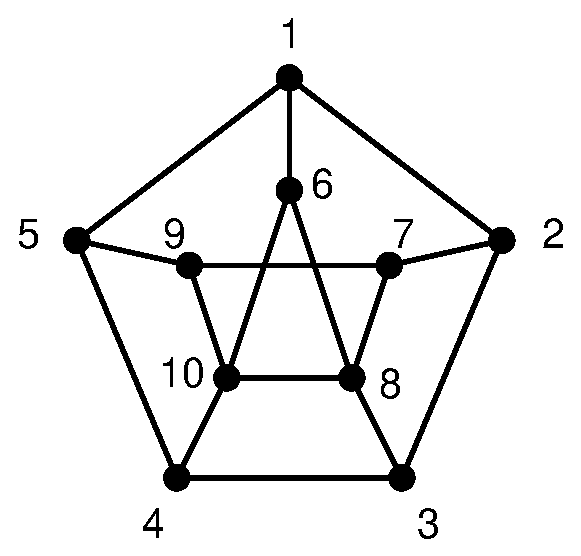
\includegraphics[width=1.5in,clip]{latex-macros/figures/G4}} }
\mbox{  \subfigure[$G_3$]{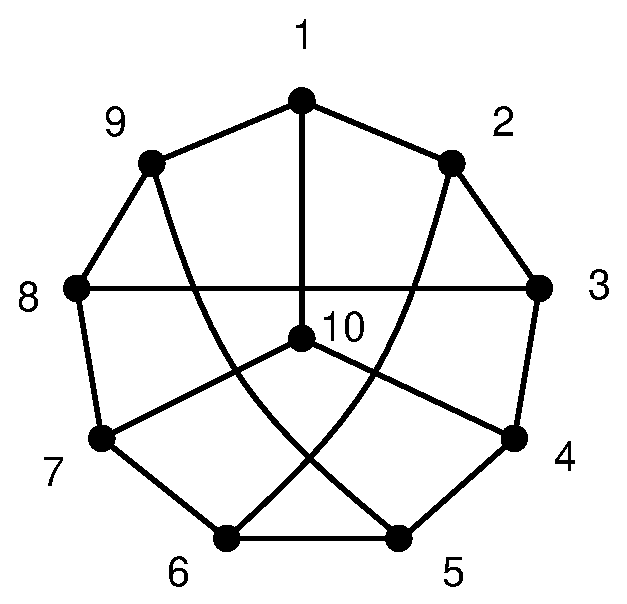
\includegraphics[width=1.5in,clip]{latex-macros/figures/G2}}
        \hspace{17mm}
        \subfigure[$G_4$]{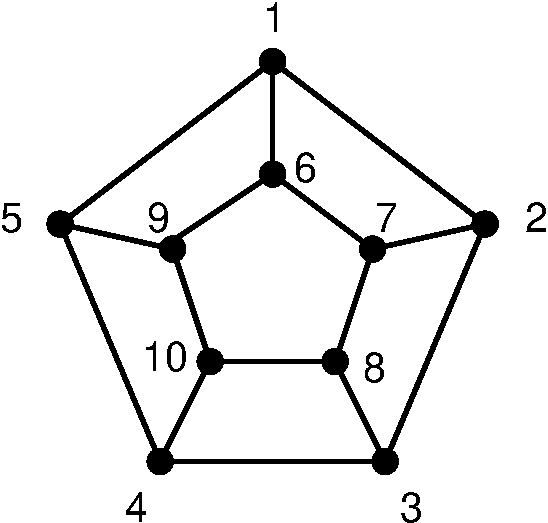
\includegraphics[width=1.5in,clip]{latex-macros/figures/G3}}
        }
\end{center}
\caption{Which graphs are isomorphic?}
\label{fig:isog}
\end{figure}

\solution{

Here, $G_1$ and $G_3$ are isomorphic.  In particular, the function
$f:V_1 \to V_3$ is an isomomorphism, where
\begin{align*}
&f(1)=1 \quad&& f(2)=2 \quad&& f(3)=3 \quad&& f(4)=8 \quad&& f(5)=9 \\
&f(6)=10 \quad&& f(7)=4 \quad&& f(8)=5 \quad&& f(9)=6 \quad&& f(10)=7
\end{align*}

$G_1$ and $G_4$ are not isomorphic to $G_2$: $G_2$ has a vertex of degree
four and neither $G_1$ nor $G_4$ has one.

$G_1$ and $G_4$ are not isomorphic: $G_4$ has a simple cycle of length
four and $G_1$ does not.

}

\end{problem}
\end{document}
